\documentclass{standalone}
\usepackage{pgfplots}
\usetikzlibrary{shapes.geometric, intersections}
\pgfplotsset{compat=1.7}

\begin{document}
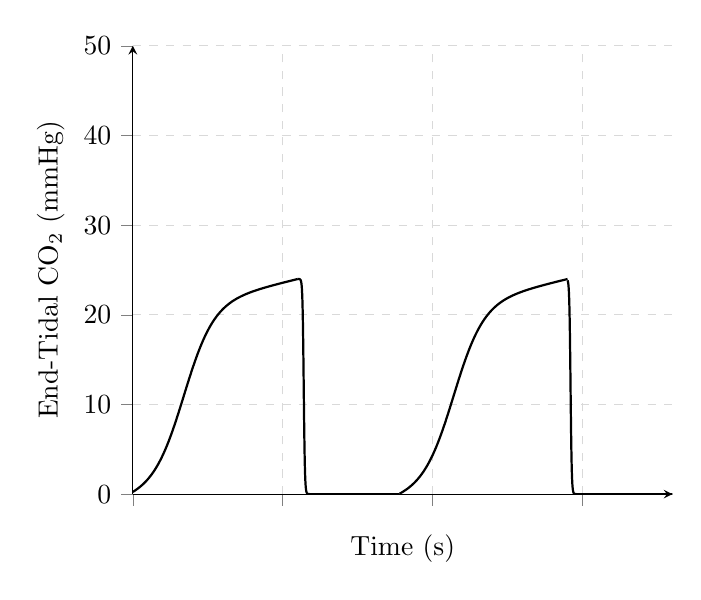
\begin{tikzpicture}

    \begin{axis}[
axis x line=bottom,
  axis y line=left,
	ymin = 0,
	ymax = 50,
	xmin = 0,
xmax = 180,
        grid = major,
        grid style={dashed, gray!30},
	 ylabel near ticks,
	xlabel near ticks,
	xticklabels={},
        xlabel=Time (s),
        ylabel=End-Tidal CO\textsubscript{2} (mmHg),
        tick align=outside,
        enlargelimits=false,]

 \addplot[domain=0:55, black, thick,samples=500] {20*(1/(1+exp(-0.2*(x-17))))+0.08*(x-5)};
 \addplot[domain=55:89, black, thick,samples=500] {24*(1/(1+exp(5*(x-57))))};

 \addplot[domain=89:145, black, thick,samples=500] {20*(1/(1+exp(-0.2*(x-107))))+0.08*(x-95)};
 \addplot[domain=145:180, black, thick,samples=500] {24*(1/(1+exp(5*(x-146))))};

%\draw[black, thick] plot[smooth,tension=0.3] coordinates { (axis cs: 0,1) (axis cs: 10, 1) (axis cs: 15,15) (axis cs: 20, 33) (axis cs: 25,35) (axis cs: 40, 37) (axis cs: 42,5) (axis cs: 45,1)};



\end{axis}

\end{tikzpicture} 
\end{document}